%-------------------------------------------------------------------------------
%	PACKAGES AND OTHER DOCUMENT CONFIGURATIONS
%-------------------------------------------------------------------------------

%------------------------------------------------
% BASIC CLASS FILE
%------------------------------------------------

\documentclass{style}

%------------------------------------------------
% ADDITIONAL OPTIONAL STYLE FILES
%------------------------------------------------

\usepackage{graphicx}
\usepackage{tabularx}
\usepackage{amssymb,amsfonts,amsmath}

%------------------------------------------------
% DO NOT EDIT THIS SECTION
%------------------------------------------------

\begin{document}

%-------------------------------------------------------------------------------
%	TITLE AND AUTHORS
%-------------------------------------------------------------------------------

\title{Context-based configuration management: \linebreak
    state of the art and challenges}

%------------------------------------------------

\author{Ghislain Loaec\affil{1}{University of Burgundy}}

\contributor{Submission Candidate}

%-------------------------------------------------------------------------------

\setcounter{secnumdepth}{3}
\maketitle % The \maketitle command is necessary to build the title page

\begin{article}

%-------------------------------------------------------------------------------
%	ABSTRACT, KEYWORDS AND ABBREVIATIONS
%-------------------------------------------------------------------------------

\begin{abstract}
The fundamental objective of ubiquitous computing is to ease the human labor in
computer use.  This results in enhancing the resources available throughout the
physical environment.  In order to extract the maximum benefit of a digital
environment, embeded systems and services must cooperate. Software failures due
to configuration errors are commonplace as computer systems continue to grow
larger and more complex. The primary challenge with context-handling
interacting with humans, is that there is no standard, or reusable model that
can be used to handle context.
\end{abstract}

%------------------------------------------------

\keywords{Context-Aware | Configuration Management}

%------------------------------------------------

\abbreviations{
  CAD, context-aware deployment;
  OMG, object management group;
  CCM, COBRA commponent model;
}

%-------------------------------------------------------------------------------
%	PUBLICATION CONTENT
%-------------------------------------------------------------------------------

\section{Introduction}

\dropcap{S}oftware configuration imposes a major cost on system administration.
Configuration errors may result in security vulnerabilities, application
crashes, severe disruptions in software functionality, unexpected changes in the
UI, and incorrect program executions. Dealing with context seems to be a major
challenge which the field of Artificial Intelligence (AI) will have to face in
the next few years. 

A context-aware system must be capable of mimicking a human’s ability to
recognise and exploit implicit information in the environment, in order to
advance or correct the operations of its functionalities.  This entails a
dynamic configuration for every component of a context-aware system, in order
to adjust its behavior depending on the situation. Although identifying and
deducing a human activity is a challenge, it is critical that context-aware
applications should operate by conveying the appropriate information to the
right place at the right time through inferring the user’s intention.
Context-aware computing is a computing paradigm in which applications can
discover and take advantage of contextual information such as location, time of
day, people and devices, and user activity.

In this paper, we present common architecture principles of context-aware
systems and derive a layered conceptual design framework to explain the
different elements common to most context-aware architectures. Based on these
design principles, we introduce various existing context-aware systems focusing
on context-aware middleware and frameworks, which ease the configuration of
context-based applications and services.

\section{Background}

Much debate has occured and are still taking place about the meaning of both
context and context aware computing.  While most people tacitly understand what
context is, they find it hard to elucidate. 

\begin{quotation}
  ... any information the can be used to charaterize the situation of an entity.
  An entity is a person, place or object that is considered relevant to the
  interation between a user and an application, including the user and the
  application themselves.  \cite{Abowd1997}
\end{quotation}

This definition makes it easier for an application developer to enumerate the
context for a given application scenario. If a piece of information can be used
to characterize the situation of a participant in an interaction, then that
information is context.

The Five Ws are questions whose answers are considered basic in
information-gathering. They constitute a formula for getting the complete story
on a subject. According to the principle of the Five Ws, a report can only be
considered complete if it answers these questions starting with an interrogative
word:

\begin{itemize}
    \item \textbf{Who} is it about?
    \item \textbf{What} happened?
    \item \textbf{When} did it take place?
    \item \textbf{Where} did it take place?
    \item \textbf{Why} did it happen?
\end{itemize}

Each question should have a factual answer — facts necessary to include for a
report to be considered complete. Importantly, none of these questions can
be answered with a simple "yes" or "no".

\begin{quotation}
  Context-aware computing : exploit the progress in sensing and mechanisms for
  observing the environement to systematically collect implict context
  \cite{Abowd2002}
\end{quotation}

This context information can be formed into an abstract model of all
actors in a system.

Context-aware computing was first defined by Schilit and Theimer as any system
that "adapts according to its location of use, the collection of nearby people
and objects, as well as changes over time" \cite{Schilit1994}
Since then, there have been numerous attempts to define context-aware
computing, most of which have been too specific

\section{Context overview}

\begin{quotation}
  Context is effective only when shared \cite{Winograd2001}. 
\end{quotation}

To ensure context is shared, context must first be gathered and managed by a
context-aware system.  This implies that the context-aware system must
understand what context is before it can go on seeking and categorising this
information. 

\subsection{Classes of context}

Schilit et. al. propose the following classification of context information:
\cite{Schilit1994}

\begin{itemize}
  \item \textbf{Computing Context} - network connectivity, bandwidth, and nearby
          resources such as printers, displays, or workstations.
  \item \textbf{User Context} - the user’s profile, location, nearby people, and
          current social situation. 
  \item \textbf{Physical Context} - lighting, noise level, traffic conditions,
          temperature.
\end{itemize}

Each of these categories contains a wealth of information relevant to the
context-aware system.  They cannot however be used in isolation to full effect.
The intention of the context-aware system is to gather and merge them together
in order to achieve an overall picture of the situation.  After the context is
stored in a buffer or repository, the system will decide then what is relevant
to the user at the present moment.

Context information may alternatively be subdivided into two categories:
physical context and virtual context.

\subsubsection{Virtual context}

The virtual context may include the version of the operating system, the
interface capabilities, the wireless technology used to accomplish
communication, email messages sent and received, and documents edited. 

\subsubsection{Physical context}

The physical context on the other hand may be the presence of another entity, be
it a user or device, the proximity to a particular printer, information
indicating if the user is standing, walking or sitting or the current weather
conditions. This entity can be summarized as any acquirable data by the use of a
sensor : lighting, noise level, traffic conditions, temperature (cf. 3.6)

\subsubsection{Historical context}

The contexts stored accross a time span. Considered to be useful but rarely
used except for mobile applications. The system must decide what historical
information is worthy of being kept. The evaluation the historical information
is prohibitively costly and so requires very efficient algorithms 

\subsection{Context information characterisics}

Researchers at the University of Queensland have classified four
characteristics: \cite{Catharina2002}

\begin{enumerate}
    \item \textbf{Context information exhibits a range of temporal
            characteristics}

            Context has already been subdivided into physical and virtual
            environement ; it can be furthermore categorized into :

            \begin{itemize}
                \item Static information : any information related to the user's
                        environement that is invariant.
                \item Dynamic information : must be accumulated continuously,
                        frequently and automatically.
            \end{itemize}

            Additionally, past context information may be needed to understand
            the full state of the environment

    \item \textbf{Context information is imperfect}

            This considers the validity of context, in particular dynamic
            context information.  The speed at which the context information
            changes raises reasons for the doubt over the soundness of the
            context.  This "delay between the production and use of context
            information" \cite{Catharina2002} is a concern.  Other sources of
            concern regarding the soundness of context information include the
	    reliability of information from the context producers : sensor
	    failure, broken path between producers or any source that would
	    provide wrong or outdated information.

    \item \textbf{Information has many alternative representations}

            The raw data gathered from both physical and virtual environment can
            take on many forms and must be processed when combined with other
            context informations.  The probability of the context-aware system
            obtaining a 100\% success rate in "capturing the relationships that
            exist between the alternative representations"
            \cite{Catharina2002} of the context information and the one apt
            to the current situation is extremely low.

    \item \textbf{Context information is highly interrelated}

            Context information derived from a particular origin may have a very
            close link with its source, so much so that it is dependant on the
            origin. 
            Context may not be reliable
            “where the characteristics of the derived information are intimately
            linked to the properties of the information it is derived from”
            \cite{Catharina2002}.

\end{enumerate}

\subsection{Context-aware system}

A system is context-aware if it uses context to provide relevant information
and/or services to the user, where relevancy depends on the user’s task.
Context-aware systems can be implemented in many ways, but in order to
accomplish this objective, the context aware system generally must :

\begin{itemize}
    \item Gather the information
    \item Serialize this information
    \item Merge the information to generate higher context
    \item Automatically take action based on the retrieved information
    \item Make the information available to the user, immediately, in the future,
            or when it is required to enhance and aid in he completion if the
            user's task.
\end{itemize}

The researchers of the Context Toolkit at the University of Berkeley propose
that there are three features that a context-aware application must support:
\cite{Dey2000}

\begin{enumerate}
    \item Presentation of information and services to a user 
    \item Automatic execution of a service for a user 
    \item Tagging of context to information to support later retrieval
\end{enumerate}

The developers of Kimura System have designed distributed components of a
pervasive context-aware system. These components fall into three classes
\cite{Voida2002}, these are: 

\begin{enumerate}
    \item Context Acquisition - the system gathers context information and adds
            it to a repository. 
    \item Context Interpretation - the system converts the gathered context
            information into a working context.
    \item User Interaction, the system displays the working context to the user
\end{enumerate}

\subsection{Gathering context information}

Some context information is explicitly given to the system, such as user's
name, age, email, environement variables or regirstry. Other primitive physical
information such as light, heat, pressure readings can be aquired through the
use of sensors

Location and identity are the most frequently sensed pieces of context. 

\begin{quotation}
Sensors are not always 100\% accurate or reliable, particularly if they are
disposable. The information gathering system must be tolerant of sensor failure,
and any information gathered from sensors must be subjected to sanity checks to
help verify its correctness. Sensor fusion is one method of avoiding this
difficulty \cite{Schmidt1999}
\end{quotation}

Let's take for instance a power plant, with several sensor which gives the
context information of temperature. The system must take some descision wether
to cool generously the reactor or not. The consequences of an
underestimation of the temperature would be catastrophic. It might be prudent
either to simply average the results and  discard reported values
that differ too greatly from what other sensors report. This method would avoid
drastic measures being taken by the context system to correct what it considers
to be temperature variations but are actually simply the result of sensor
failure. 

\subsection{Retrieving context information}

\begin{itemize}
  \item Push Model - The context source gather the context information before it
          is needed. It gives better performances but requires large and frequent
          resource consumption for some information the may never be exploited.
  \item Pull Model - Collects only the context information that is required
          It allows to get the information on demand but is exposed to network
          delays and services unavailability
\end{itemize}

The method of context-data acquisition is very important when designing
context-aware systems because it predefines the architectural style of the
system at least to some extent. Chen (2003) \cite{Chen2003} presents three
different approaches on how to acquire contextual information.

\subsubsection{Direct sensor access}

This approach is often used in devices with sensors locally built in. The client
software gathers the desired information directly from these sensors, i.e.,
there is no additional layer for gaining and processing sensor data. Drivers for
the sensors are hardwired into the application, so this tightly coupled method
is usable only in rare cases. Therefore, it is not suited for distributed
systems.

\subsubsection{Middleware infrastrucure}
 
The middleware based approach introduces a layered architecture to context-aware
systems with the intention of hiding low-level sensing details.
This approach is equivalent to client-server model, more flexible the widget
since it promotes the independence of each components in the context-aware
system. Every component must be able to perform the following functionnalities :
establishing connections, organising input and output messages and managing
faults.  This model is significantly more complex but the approach is pretty
straightforward since it supports large range of device and application using
standard coding and networking protocols.

\subsubsection{Context server}

This distributed approach extends the middleware based architecture by
introducing an access managing remote component. Gathering sensor data is moved
to this so-called context server to facilitate concurrent multiple access

\subsection{Achitectures for Managing Context}

Winograd (2001) \cite{Winograd2001} describes three different context management
models for coordinating multiple processes and components:

\begin{itemize}
        \item \textbf{Widgets}
                The key objective of the widget is to seperate the application
                from the context aquisition issues in order to abstract the
                complexity of collecting and managind the context information.
                The widget is used as a mediator to pass only the pertinent
                information to the application, A context widget functions
                independently of applications, which permits multiple
                applications to use it simultaneously. A context widget is also
                responsible for maintaining a complete history of the context
                aquiered for the user's situation.  It remains the most
                prevalent model.

        \item \textbf{Network services}
                This more flexible approach, argued for example in Hong and
                Landay (2001) \cite{Hong2001}, resembles the context server
                architecture.  Instead of a global widget manager discovery
                techniques are used to find networked services. This service
                based approach is not as efficient as a widget architecture due
                to complex network based components but provides robustness.

        \item \textbf{Blackboard}
                In contrast to the process-centric view of the widget and the
                service-oriented model, the blackboard model represents a
                data-centric view The blackboard model adopts a data-centric
                point of view, matching a specified patterns in data. In this
                asymmetric approach processes post messages to a shared media,
                the so-called blackboard, and subscribe to it to be notified
                when some specified event occurs. Advantages of this model are
                the simplicity of adding new context sources and the easy
                configuration.
\end{itemize}

\subsubsection{Trade-off criteria}

When deciding on the most suitable model for a context aware system, we want to
consider the trade-off characteristics : 

          \begin{itemize}
            \item Efficiency : accelerate the throughput of information
                    considering the the bandwidth and latency caused by the
                    explosion in the number of networked applications and
                    devices.
            \item Effort in configuring : considering te various amount of
                    components, perform a change in the configuration
                    state, without the disruption or total failure of the
                    system, it not a tedious task. This model must make
                    sure the edit is safe.
            \item Robustness : the degree to which the system can cope with
                    failure
            \item Simplicity : 
                    \begin{quotation}
                      a system that requires complex understanding by system
                      builders in order to make use of its facilities will be
                      used only by those who have the dedication and motivation
                      to master it.  \cite{Winograd2001}
                    \end{quotation}
            \item Extensibility : 
                    \begin{quotation}
                      services supporting a general notion of context must be
                      easily extensible to accommodate new and unanticipated
                      sources of context information.  \cite{Ebling2002}
                    \end{quotation}
          \end{itemize}

The trade-offs can be used to compare and contrast the different models for
context management. 

\begin{quotation}
        The widget model has tight coupling of system components, which may make
        it the most efficient model in some circumstances, however it suffers
        from complex configuration and issues with powerlessness in the cause of
        failure. The infrastructure model with its independent components may be
        extremely complex, which is a no factor for many developers, however its
        positive criteria of straightforward configuration and robustness may
        compensate for the negative implication of complexity. Finally the
        blackboard model with its very loosely coupled components may suffer
        from efficiency problems, but it is a simple, robust, easily
        configurable model. \cite{Winograd2001}
\end{quotation}

\subsection{Representing Context}

There are several ways to modelize context information :

\begin{itemize}
    \item Key-Value : simplest data structure for context modelling. They are
            frequently used in various service frameworks, where the key-value
            pairs are used to describe the capabilities of a service
    \item Markup scheme : hierarchical data structure consisting of markup tags
            with attributes and content. Profiles represent typical
            markup-scheme models.
    \item Graphical : Unified Modelling Language (UML), extension to the
            Object-Role Modelling (ORM) by context
    \item Object oriented : use the full power of object orientation (e.g.,
            encapsulation, reusability, inheritance). Existing approaches use
            various objects to represent different context types (such as
            temperature, location, etc.), and encapsulate the details of context
            processing and representation
    \item Logic based : high degree of formality. Typically, facts, expressions
            and rules are used to define a context model. A logic based system
            is then used to manage the aforementioned
    \item Ontology based : represent a description of the concepts and
            relationships. very promising instrument for modelling contextual
            information due to their high and formal expressiveness and the
            possibilities for applying ontology reasoning techniques
\end{itemize}

Conclusion of the evaluation presented in Strang and Linnhoff-Popien
\cite{Strang2004}, based on six requirements, show that ontologies are the most
expressive models and fulfil most of their requirements.

Korpipää et al. \cite{Korpipaa2003} present some requirements and goals having
designed a context ontology:

\begin{itemize}
    \item Simplicity: the used expressions and relations should be as simple as
            possible to simplify the work of applications developers
    \item Flexibility and extensibility: the ontology should support the simple
            addition of new context elements and relations
    \item Genericity: the ontology should not be limited to special kind of
            context atoms but rather support different types of context
    \item Expressiveness: the ontology should allow to describe as much context
            states as possible in arbitrary detail.
\end{itemize}

A single context atom can be described with a couple of attributes. The two most
obvious are:

\begin{itemize}
        \item Context type : category of context such temperature, time, speed,
                etc. This type information may be used as a parameter for a
                context query or a subscription.
        \item Context value : raw data gathered by a sensor. The unit depends on
                the context type and the applied sensor, e.g., degree Celsius,
                miles per hour, MegaByte etc.
\end{itemize}

Context type and context value are not enough information to build a working
context-aware system. Additional attributes that might be useful include:

\begin{itemize}
        \item Time stamp : date/time-value describing when the context was
                sensed. It is needed e.g., to create a context history and deal
                with sensing conflicts.
        \item Source : how the information was gathered. In case of a hardware
                sensor it might hold the ID of the sensor and allow an
                application to prefer data from this sensor.
        \item Confidence : the uncertainty of this context type. Not every data
                source delivers accurate information, e.g., location data
                suffers inaccuracy depending on the used tracking tool
\end{itemize}

\subsection{Interpreting the context}

\begin{quotation}
        Interpretation refers to the the process of raising the level of
        abstraction of a piece of context
        \cite{Dey2001}
\end{quotation}

After sensing, acquiring and saving the context from various sources the next
activity for the context- aware system is to produce a mechanism for achieving
context interpretation, so that the gathered context information is utilised in
a fitting manner.  The interpretation may involve integrating numerous contexts
into one to provide a higher-level context, thus the interpreter alters context
information by raising its level of abstraction.  One approach is to use context
fusion to convert the lower level context into higher level usable by
applications. \cite{Dustdar2007}

\subsection{Layered conceptual framework}

\begin{itemize}
        \item Application
        \item Storage management
        \item Preprocessing : 
                \begin{itemize}
                        \item Translation : not implemented in every
                                context-aware system but may offer useful
                                information if the raw data are too coarse
                                grained. The preprocessing layer is responsible
                                for reasoning and interpreting contextual
                                information
                        \item Aggregation / Composition : consisting of several
                                different context data sources, the single
                                context atoms can be combined to high-level
                                information in this layer 
                \end{itemize}
        \item Raw data retrieval :
                appropriate drivers for physical sensors and APIs for virtual
                and logical sensors. The query functionality is often
                implemented in reusable software components which make low-level
                details of hardware access transparent by providing more
                abstract methods such as getPosition().
        \item Sensors :
                \begin{itemize}
                        \item Physical sensors : hardware sensor to capture
                                physical data
                                \begin{itemize}
                                        \item Light
                                        \item Visual context
                                        \item Audio
                                        \item Motion / acceleration
                                        \item Location
                                        \item Touch
                                        \item Temparature
                                        \item Physical Attributes
                                \end{itemize}
                        \item Virtual sensors : source context data from
                                software applications or services tracking
                                systems, electronic calendar, travel-booking
                                system, mouse mouvement, etc.
                        \item Logical sensors : physical + virtual + additional
                                information from databases in order to solve
                                higher tasks
                \end{itemize}
\end{itemize}

\subsection{Security and Privacy}

\begin{quotation}
	Privacy is intrinsically bound up with control \cite{Ackerman2001}
\end{quotation}

As context may include sensitive information on people, e.g., their location and
their activity, it is necessary to have the opportunity to protect privacy.
Context-aware systems raise privacy challenges not previously considered by
traditional systems.  The control of the various sensors and services is not
well specified in Dey et al. \cite{Dey2001}, although often applications such as
Context Toolit are implied to be under the control of a "user".  Users are
assigned to sensed context data as their respective owners. They are allowed to
control the other users’ access. 

However, the control over systems determining the presence of individuals in a
room or other location, on the other hand, is not specified at all. This is a
critical point.

In general, in a context aware environment with a suite of context aware
applications, an individual operates within many social environments, and social
environments may make a use of many individuals' data.

Often disregarded aspects, security and privacy belong to the most important
components of a context-aware system as the protection of sensitive context data
must be guaranteed.

\section {Existent systems and frameworks}

In Table 1 we have summarised the main aspects of the discussed approaches. The
architectural style of a context-aware system is mainly driven by the context
acquisition method. The main criteria for a reasonable architectural approach
is the separation of concerns between the context acquisition and the user
components as proposed by Dey (2000) \cite{Dey2000}. All the frameworks
presented in this paper support this separation of concerns.

\begin{table*}%[h]
    \begin{tabularx}{\linewidth}{
      >{\raggedright\arraybackslash}X
      >{\raggedright\arraybackslash}X
      >{\raggedright\arraybackslash}X
      >{\raggedright\arraybackslash}X
      >{\raggedright\arraybackslash}X
      >{\raggedright\arraybackslash}X
      >{\raggedright\arraybackslash}X
      >{\raggedright\arraybackslash}X
    }
        \hline
        \textbf{Architecture} & 
        \textbf{Sensing} & 
        \textbf{Context model} &
        \textbf{Context processing} &
        \textbf{Resource discovery} &
        \textbf{Historical Context data} &
        \textbf{Security and privacy} & 
        \\
        \hline
        CASS &
        Centralized Middleware &
        Sensor nodes &
        Relational data model &
        Inference engine and knowledge base &
        n.a. &
        Available &
        n.a.\\

        Cobra &
        Agent based &
        Context acquisition module &
        Ontologies (OWL) &
        Inference engine and knowledge base &
        n.a. &
        Available &
        Rei policy language\\

        Context Management Framework &
        Blackboard based &
        Resource servers &
        Ontologies (RDF) &
        Context recognition service &
        Resource servers + subscription mechanism &
        n.a &
        n.a.\\

        Context toolkit &
        Widget based &
        Context widgets &
        Attribute-value tuples &
        Context interpretation and aggregation &
        Discoverer component &
        Available &
        Context ownership\\

        CORTEX &
        Sentient object model &
        Context component framework &
        Relational data model &
        Service discovery framework &
        Resource management component framework &
        Available &
        n.a.\\

        Gaia &
        MVC (extended) &
        Context providers &
        4-ary predicates (DAML + OIL) &
        Context-service module (first-order logic) &
        Discovery service &
        Available &
        Supported (e.g., secure tracking, location privacy, access control)\\

        Hydrogen &
        Three layered architecture &
        Adapters for various context types &
        Object-oriented &
        Interpretation and aggregation of raw data only &
        n.a. &
        n.a. &
        n.a.\\

        SOCAM &
        Distributed with centralized server &
        Context providers &
        Ontologies (OWL) &
        Context reasoning engine &
        Service locating service &
        Available &
        n.a.\\

        \hline
    \end{tabularx}
    \caption{Comparison of existing context-management frameworks}
    \label{ContextManagementFrameworkComparison}
\end{table*}

\begin{figure}[h]
    \centerline{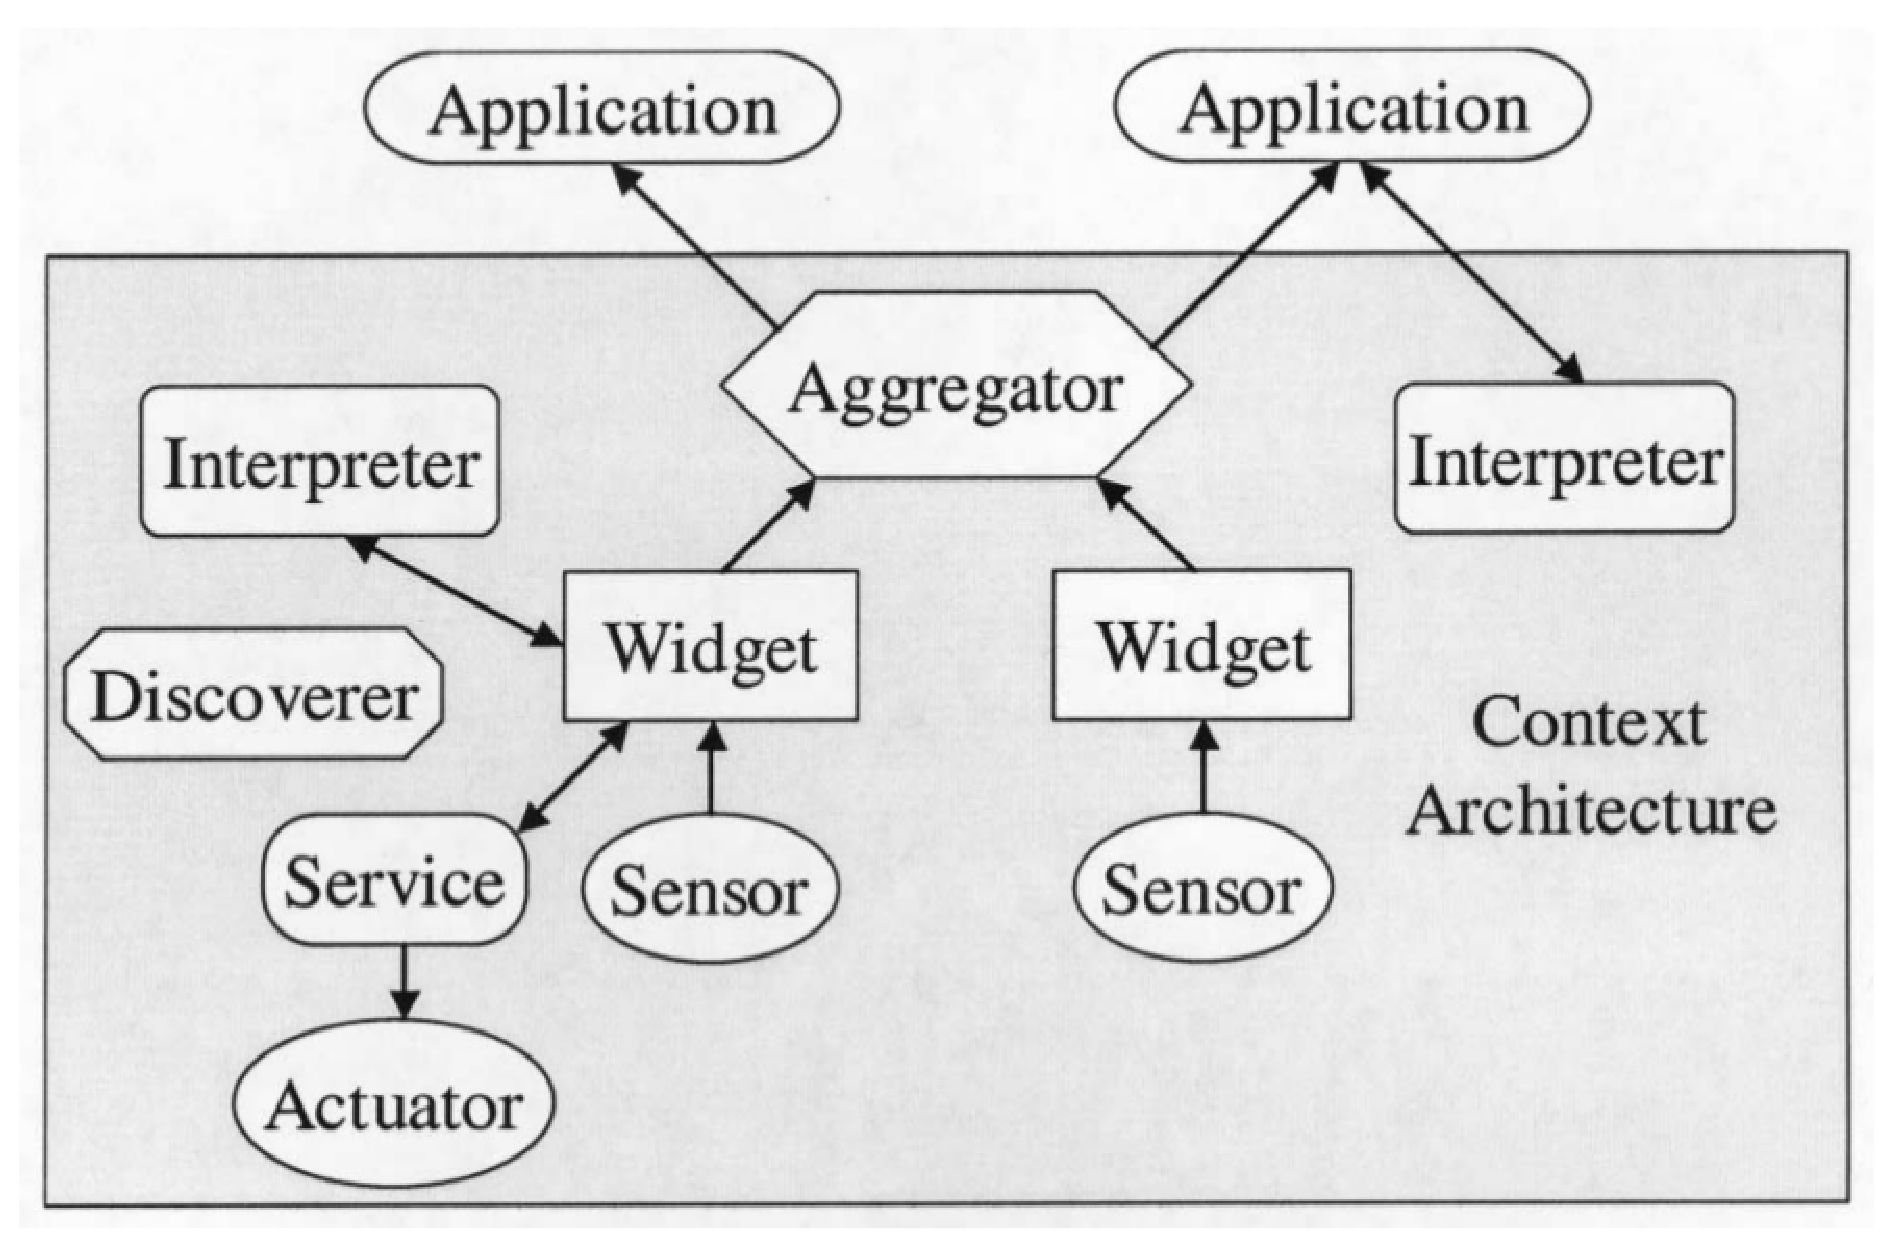
\includegraphics[width=0.6\linewidth]{img/context_toolkit.eps}}
    \caption{Example configuration of context toolkit components}
    \label{Contexttoolkit}
\end{figure}

\subsection{Sensing technologies}

In every framework, the sensing technology is implemented differently. In order
to support the aforementioned separation of concerns, it is important to
encapsulate the concrete sensing mechanism in separate components. Furthermore,
it allows to access the contextual data via defined interfaces. There is so far
no standard description language or ontology to enable the reuse of contextual
information accross various middleware systems and frameworks. Therefore,
proprietary solutions have emerged, as used by many frameworks.
For sensing the context information SOCAM has the most sophisicated approach :
web services provide apis (using SOAP) for external virtual sensors and internal
providers for querying sensores are consumed by using context events. Those
context events are modelized in OWL based on a prefefined ontology.

\subsection{Context representations}

For providing intelligent and adaptable context-aware applications or services,
the context model and the context processing logic supported by individual
frameworks is a major criteria. Ontologies provide a rich formalism for
representing context information. Based on a highly sophisticated ontological
model, the reasoning engines can derive new concepts to adapt the service
behaviour accordingly. The key-value context representation used in Context
Toolkit is, therefore, a major drawback. The fact that such attributes do not
hold any semantics rescricts consequently the development of intelligent context
processsing and aggregation. In addition, non-ontology based model requires a 
consequent programming effort and tightly couples the context model to the rest
of the system. Moreover, the reasoning and knowledge sharing across systems are 
impossible due to the lack of declarative semantics of programs. SOCAM, for
instance, uses a general upper ontology to specify basic common contextual
properties and to refine this general ontology. In order to provide very fine
grained possibilities for specifying and formalising context, some
domain-specific ontologies can be defined.

\subsection{Resource discovery}

Resource discovery mechanisms are rarely implemented despite the importance of
such dynamic mechanisms, especially in a pervasive environment, where the
context sources and available sensors change constantly. SOCAM is the only
system based the service oriented architecture.  It offers a service
locating service, which dynamically binds to available context providers. This
missing feature in most frameworks is indeed a consequent shortcomming since
it implies that the used context sources are stable and permanently available,
which is not always the case in real-world applications. If one or more context
sources behave wrong, it may lead to a decreased availability of the
context-aware service or application. 

\subsection{Historical context management}

Although most frameworks keep a history of context data, none of them actually
exploits it. Yet, It could allow to provide highly adaptable context-aware
services if historical context was used to implement self-learning algorithms.
Furthermore, contextual information can be predicted to proactively provide a
certain set of services to the user.

\subsection{Security and privacy}

Another important aspect is security and privacy.  Contextual information mostly
considers user profile information and other sensitive information.  Therefore,
concepts are needed to express policies and to define ownership of context
information. CoBrA includes an own flexible policy language to control context
access, called Rei \cite{Kagal}. This policy language is modelled on deontic
concepts of rights, prohibitions, obligations and dispensations and controls
data access through dynamically modifiable domain dependent policy rules.
Gaia uses several mechanisms to define privacy restrictions and secure
communication for tracking locations of people. The Context Toolkit implements
the concept of context ownership, which is used to allow access to the context
to the owner only. Security concepts are not implemented in the other frameworks.
Many systems totally lack security modules, others offer basic security
mechanisms and only a few systems provide advanced and sufficient security
options. 

\subsection{Conclusion}

Every system and framework uses its own format to describe context and
its own communications mechanisms which appears to be the main problem of
today's context-aware systems.
%\subsection{Location-based systems}
%
%GPS satellites, mobile phone towers, badge proximity detectors, cameras,
%magnetic card readers, barcode readers, etc.
%
%\subsection{Context-aware systems}
%
%Use only one aspect of context, namely location information.  The use of
%different types of context atoms such as noise, light and location allows the
%combination to high-level context objects.
%
%\subsection{Context-aware architectures}
%
%CaSS : Context-Awareness Sub-Structure
%
%\begin{itemize}
%        \item CADeComp : Context-aware deployment of component-based
%                applications
%        \item CaSS : Context-Awareness Sub-Structure
%        \item CoBrA : Context Broker Architecture
%        \item SOCAM : Service-Oriented Context-Aware Middleware
%
%        \item CORTEX : context-aware middleware approach. The architecture is
%                based on the Sentient Object Model
%        \item Gaia : another middleware infrastructure, extends typical
%                operating system concepts to include context-awareness.
%        \item Context Management Framework : Blackboard based
%        \item Context Toolkit : Widget based
%        \item Hydrogen : Three layered architecture, adapters for various
%                context type
%        \item ...
%\end{itemize}

\section{Research directions and challenges}

In this paper we described different design principles and context models for
context-aware systems and presented various existent middleware and
server-based approaches to ease the configuration of context-aware application.

There are several research areas involved in the development of context-based
configuration. Here are three of the most relevant :

\subsection{Middleware and implementation details}

The need for new middleware arises on the implementation side. Current
middleware technologies are not adequate to handle the resctrictions imposed by
mobility and smart environmental systems : volatile connections, processing and
memory restrictions on mobile devices, narrow communication channels, reduced
screens, restricted input mechanisms, and the list goes on. There are a set of 
contex-aware imlementations in litterature with some working prototypes :

\begin{itemize}
    \item \textbf{Hydrogen} \cite{Hofer2002}: a three layer architecture
    \item \textbf{Gaia} \cite{Chetan2005}: another middleware infrastructure,
    extends typical operating system concepts to include context-awareness.
    \item \textbf{CybreMinder} \cite{Abowd2002}: a context-aware system for sup-
    porting reminders
    \item \textbf{Context Toolkit} \cite{Dey2001}: a widget based architecture
\end{itemize}

\subsection{Representation of context-information}

The representation of context-information is another concern. We presented in
this paper a generic ontology approach. It is based on four main concepts: user,
environment, platform and resources.  Presently, ontologies are mainly employed
to enable communication across the different devices in the same network. As
proposed by ContextUML \cite{Sheng2005}, the Unified Modeling Language (UML) can
also be used to model context. The models could be used to separate the
definition and information related to the context from the specific
implementation. There are other characteristics that make context information
difficult to model, as stated before, it is sometimes necessary to differentiate
between static and dynamic information.

\subsection{Semantic rules}

Another area of research would be concerning use of rules to express behavior in
terms of high-level elements. Rule languages are used in some cases to achieve
context-awareness.  CRIME \cite{Mostinckx2007} for example, is a prototypical
implementation of the Fact Space Model, which is a coordination language that
provides the applications a view of their environment The rules in CRIME
describe the behavior of the applica- tions according to the context
information. CRIME also deals with disconnection by invalidating the facts and
the conclusions that are drawn from devices that are no longer available in the
environment

\section{Conclusion and discussion}

Component technologies will play a fundamental role in the next generation
computer systems as the complexity of software and the diversity and
pervasiveness of computing devices increase. However, component technologies
must offer mechanisms for automatic management of inter-component dependencies
and component-to-resource dependencies. Otherwise, the development of
component- based systems will continue to be difficult and frequently lead to
unreliable and non-robust systems.  

Future ubiquitous computing environments will be composed of thousands of
devices running millions of software components. Current systems rely heavily
on manual configuration but with a system composed of millions of components
this will no longer be possible.  There are only two ways out of this
situation: static configuration or dynamic, automatic configuration

Since future environments tend to be more and more dynamic, automatic
configuration seems to be the only viable solution.

%-------------------------------------------------------------------------------
%	ACKNOWLEDGEMENTS
%-------------------------------------------------------------------------------

\begin{acknowledgments}
    The author gratefully acknowledge the help and wise input provided by Prof.
Nader Mbarek during the development of this work.  A special thank you goes to
Prof. Albert Dipanda for allowing me to work on a topic in adequacy with my
professional activities.  Thanks to Luc Bourdot, president of the FOSS center
of excellence of the french ministry of education and EOLE team leader, for
granting me some free time to work on this paper. I would to thank Gwenael
Remond as well, head developper of Era firewall, for his valuable comments and
for sharing his knowledge on autonomic configuration. I am also grateful for the
precious feedback provided by the anonymous reviewers of this paper
\end{acknowledgments}

%-------------------------------------------------------------------------------
%	LIST OF FIGURES / TABLES
%-------------------------------------------------------------------------------

%\tableofcontents
\listoffigures
\listoftables

%-------------------------------------------------------------------------------
%	APPENDICES (OPTIONAL)
%-------------------------------------------------------------------------------

\appendix[Glossary]

\begin{itemize}
        \item CADeComp : Context-aware deployment of component-based
                applications
        \item CaSS : Context-Awareness Sub-Structure
        \item CoBrA : Context Broker Architecture
        \item SOCAM : Service-Oriented Context-Aware Middleware
\end{itemize}

\appendix[References]

%-------------------------------------------------------------------------------
%	BIBLIOGRAPHY
%-------------------------------------------------------------------------------

\nocite{*}

\bibliography{biblio}{}
\bibliographystyle{plain}

%-------------------------------------------------------------------------------

\end{article}

\end{document}
